\documentclass[aps,prl,reprint,superscriptaddress,longbibliography,nofootinbib,floatfix]{revtex4-2}

\usepackage[T1]{fontenc}
\usepackage[utf8]{inputenc}
\usepackage{lmodern}
\usepackage{amsmath,amssymb,mathtools}
\usepackage{booktabs}
\usepackage{microtype}
\usepackage{siunitx}
\usepackage{xcolor}
\usepackage{tikz}
\usepackage[hidelinks]{hyperref}
\usetikzlibrary{arrows.meta,positioning,calc}

\sisetup{
    detect-all,
    round-mode = none,
    exponent-mode = input,
    exponent-product = \times,
    group-separator = {\,},
    group-minimum-digits = 4
}

\newcommand{\Padm}{P_{\mathrm{adm}}}
\newcommand{\Oadm}{\Omega_{\mathrm{adm}}}
\newcommand{\Mpl}{M_{\mathrm{Pl}}}
\newcommand{\Mplred}{\bar M_{\mathrm{Pl}}}
\newcommand{\Seam}{\Sigma}
\newcommand{\USeam}{\mathcal U_{\Seam}}
\newcommand{\alphazero}{\alpha(0)}
\newcommand{\rhoLambda}{\rho_{\Lambda}}
\newcommand{\rhoLambdaRed}{\rho_{\Lambda,\mathrm{red}}}
\newcommand{\omegadm}{\omega_{\mathrm{DM}}}

\begin{document}

\title{A Seam-Induced Cosmological Constant from the Fine-Structure Constant and the Late-Time Hubble Scale}
\author{Stefan Hamann}
\noaffiliation
\author{Alessandro Rizzo}
\noaffiliation
\date{\today}

\begin{abstract}
Under the seam-determinant identification of Conjecture 13.1, this Letter extracts only the cosmological-constant branch of TFPT and separates its status layers explicitly: imported benchmark/suite inputs, the conjectural determinant route itself, the additional admissible-branch spectral assumptions used for the leading Fredholm estimate, and the derived late-time Hubble closure. Treating $\alpha(0)$, $\Omega_b$, and $\omega_{\mathrm{DM}}=\Omega_{\mathrm{DM}}h^2$ as imported inputs, the leading Fredholm approximation with the additional lowest-block identification $m_1=\Omega_{\mathrm{adm}}=48$ gives $\delta_{\Seam}^{\mathrm{lead}}=48\,e^{-2\pi\alpha^{-1}(0)/3}=1.085\times10^{-123}$. Relative to the companion manuscript, we make the Planck-mass convention change explicit by displaying both the reduced-Planck density convention $\rho_{\Lambda,\mathrm{red}}=\bar M_{\mathrm{Pl}}^4\delta_{\Seam}$ and the unreduced-Planck density convention $\rho_\Lambda=M_{\mathrm{Pl}}^4\delta_{\Seam}$ used for late-time comparison. Under the self-consistent flatness closure, the Fredholm-leading density gives $H_0^{\mathrm{lead}}=66.51\,\mathrm{km\,s^{-1}\,Mpc^{-1}}$, while an independent discrete gap-equation suite route gives $\rho_\Lambda^{\mathrm{disc}}=2.4723\times10^{-47}\,\mathrm{GeV}^4$ and $H_0^{\mathrm{disc}}=67.10\,\mathrm{km\,s^{-1}\,Mpc^{-1}}$. The internal TFPT span $66.5$--$67.1$ thus lies $1.6\sigma$ to $0.5\sigma$ below Planck and remains far below SH0ES, so within this framework the Hubble tension is not relieved by dialing the asymptotic vacuum scale upward.
\end{abstract}

\maketitle

\section{What TFPT Is}

This Letter extracts the cosmological-constant branch of Conjecture 13.1 from the companion TFPT manuscript \cite{tfpt31}. The cosmological constant problem is the problem of explaining why the observed late-time vacuum energy is tiny in Planck units yet nonzero \cite{einstein1917,weinberg1989}; the Hubble-tension problem asks whether the mismatch between CMB-inferred and locally inferred $H_0$ points to new cosmological structure or to unresolved systematics \cite{planck2018,riess2022}. Before discussing the cosmological branch, however, the framework itself needs one short explanation.

In the language of the companion manuscript, TFPT is a carrier-first theory of admissible vacua on the oriented double cover. Its primitive datum is a relative spectral package
\[
(X,\Seam,\iota,D_{\mathrm{rel}},\mathcal H_{\mathrm{int}},f,\chi_{\mathrm{seed}})
\]
rather than an absolute vacuum-energy sum. A hard carrier theorem then selects the minimal rank-$5$ split $E_3\oplus E_2$; the closure layer upgrades admissibility to an operator projector $\Padm$; and the imported APS family theorem yields
\[
F\cong\mathbb C^3,
\qquad
N_{\mathrm{fam}}=3,
\qquad
\Oadm=48.
\]
The present Letter uses only the seam-vacuum sector of that larger architecture.

Three TFPT ideas are essential here. First, vacuum quantities are defined \emph{relatively}, by comparison to a reference sector. Second, the seam $\Seam$ carries the residual vacuum observable that survives this subtraction. Third, cosmological outputs are read only after restricting to the admissible branch selected by $\Padm$. The Letter is therefore not a full rederivation of TFPT cosmology, but a focused extraction of one mechanism inside the larger carrier-first framework.

Conceptually the TFPT setup belongs to the relative spectral-action lineage rather than to a direct zero-point summation picture \cite{connes1997}. In the present Letter the only model-specific step is the identification of the relevant seam transfer operator; once that operator is assumed to be trace class, the determinant language itself is standard Fredholm technology \cite{simon2005}. This distinction matters because it separates the mathematical control of the expansion from the physical hypothesis about what the relevant operator should be.

\begin{center}
\fbox{\parbox{0.96\columnwidth}{
\textbf{Imported objects for the Letter.}
From \cite{tfpt31} the Letter imports the admissible projector $\Padm$, the seam boundary operator $B_{\Seam}$, the admissible determinant $\det_{\mathrm{adm}}$, and the family closure
$F\cong\mathbb C^3$, $N_{\mathrm{fam}}=3$, hence
$\Oadm=N_{\mathrm{fam}}\dim S^+=3\times16=48$.
For the purposes of the short Letter, $\alpha(0)$ is treated as an imported CODATA benchmark datum, $\Omega_b$ as an imported benchmark-side baryon fraction from the companion manuscript's seed/Planck comparison layer, and $\omegadm:=\Omega_{\mathrm{DM}}h^2$ as an imported TFPT suite late-time matter input.
None of these ingredients is rederived in the Letter itself.
}}
\end{center}

Because the manuscript is now standalone, the output layers must be separated more carefully than in the previous draft. The primary Fredholm object is the dimensionless seam number
\begin{equation}
\begin{aligned}
\delta_{\Seam}
:=
-\log\det\nolimits_{\mathrm{adm}}(1-\USeam),\\
\USeam:=\Padm e^{-\ell_{\Seam}|B_{\Seam}|}\Padm.
\end{aligned}
\label{eq:delta-def}
\end{equation}
From that same seam number one may form two absolute normalizations:
\begin{equation}
\rhoLambdaRed
=
\Mplred^4\,\delta_{\Seam},
\qquad
\rhoLambda
=
\Mpl^4\,\delta_{\Seam}.
\label{eq:norm-split}
\end{equation}
The first is the reduced-Planck density convention used in the companion manuscript \cite{tfpt31}; the second is the unreduced-Planck density convention used here because the Letter compares directly to the standard vacuum-energy density scale and then to the late-time Friedmann closure. The difference is substantial,
\[
\frac{\Mpl^4}{\Mplred^4}
=
(8\pi)^2
\approx
632.0,
\]
so the two absolute normalizations must be displayed explicitly rather than silently interchanged.

In particular, Eq.~\eqref{eq:norm-split} is not a claim that the two normalizations are physically interchangeable. It is a bookkeeping statement: the companion manuscript states the seam output in reduced-Planck units, while the present Letter additionally reports the unreduced-Planck density because the late-time cosmological comparison is formulated as an energy density in the flat Friedmann equation. Displaying both conventions side by side is therefore the cleanest way to avoid a hidden patch at the numerically most sensitive point of the argument.

The load-bearing electromagnetic input is the retained low-energy coupling
\[
\alpha^{-1}(0)=137.0359992
\]
from CODATA 2022 \cite{codata2022}. In the short Letter this is treated as an imported benchmark datum, not as a fresh derivation. The companion manuscript motivates why the seam attenuation scale is tied to the retained infrared electromagnetic branch rather than to a running quantity such as $\alpha(M_Z)$, whose threshold- and scheme-dependence belong to the later RG comparison map. In the present Letter that IR choice therefore remains an imported modeling decision, but it is at least a controlled and explicit one.

\section{Fredholm Leading Route}

The seam action is fixed by
\begin{equation}
\ell_{\Seam}\lambda_1^+(B_{\Seam})
=
S_{\Seam}
:=
\frac{2\pi}{3}\alpha^{-1}(0)
\approx
287.01.
\label{eq:seam-action}
\end{equation}
For the leading route used in this Letter, one spectral point must be stated explicitly. We assume that the admissible projector reduces the seam branch used here, equivalently that $\Padm$ commutes with $|B_{\Seam}|$ on that branch, so the admissible restriction of $|B_{\Seam}|$ is diagonalized by admissible seam modes $\lambda_j^+(B_{\Seam})$. We furthermore assume that no admissible seam zero mode survives, so $\lambda_1^+(B_{\Seam})>0$ and therefore $\operatorname{Spec}(\USeam)\subset(0,1)$. Under these assumptions the eigenvalues of $\USeam$ are
\[
u_j=e^{-\ell_{\Seam}\lambda_j^+(B_{\Seam})},
\qquad
0<u_j\le e^{-S_{\Seam}}\ll1.
\]
Hence the spectral radius obeys $r(\USeam)<1$, so the Fredholm expansion converges absolutely:
\begin{equation}
\delta_{\Seam}
=
\sum_{k\ge1}\frac{1}{k}\,\mathrm{Tr}\,\USeam^k.
\label{eq:fredholm-expansion}
\end{equation}
Moreover
\begin{equation}
\begin{aligned}
\mathrm{Tr}\,\USeam
=
m_1e^{-S_{\Seam}}
\,+\!\!\sum_{j\ge2}m_j e^{-\ell_{\Seam}\lambda_j^+(B_{\Seam})},\\
m_1\ge1.
\end{aligned}
\label{eq:trace-split}
\end{equation}
For the leading route we additionally identify the lowest admissible seam-block multiplicity with the imported family-closure occupancy,
\[
m_1=\Oadm=48.
\]
That identification is an imported/conjectural bridge step in the Letter, not a deduction carried out inside the short paper. With that explicit status understood, the leading Fredholm approximation is not merely "small"; it is controlled by the lowest admissible block together with the gap to higher seam modes.

\begin{figure}[t]
\centering
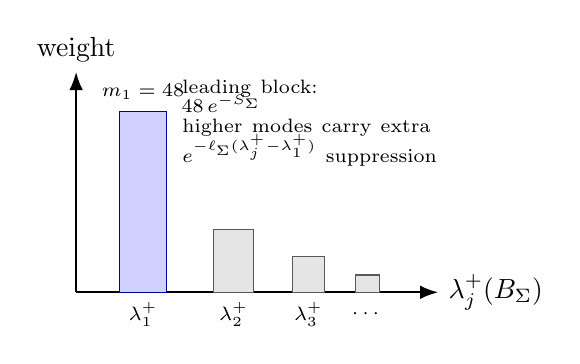
\begin{tikzpicture}[>=Latex]
\draw[->, thick] (0,0) -- (4.6,0) node[right] {$\lambda_j^+(B_{\Seam})$};
\draw[->, thick] (0,0) -- (0,2.8) node[above] {weight};
\filldraw[fill=blue!18, draw=blue!60!black] (0.55,0) rectangle (1.15,2.3);
\filldraw[fill=gray!20, draw=gray!70!black] (1.75,0) rectangle (2.25,0.8);
\filldraw[fill=gray!20, draw=gray!70!black] (2.75,0) rectangle (3.15,0.45);
\filldraw[fill=gray!20, draw=gray!70!black] (3.55,0) rectangle (3.85,0.22);
\node[align=center] at (0.85,2.55) {\scriptsize $m_1=48$};
\node[align=center] at (0.85,-0.28) {\scriptsize $\lambda_1^+$};
\node[align=center] at (2.00,-0.28) {\scriptsize $\lambda_2^+$};
\node[align=center] at (2.95,-0.28) {\scriptsize $\lambda_3^+$};
\node[align=center] at (3.70,-0.28) {\scriptsize $\cdots$};
\node[align=left, text width=3.6cm] at (3.15,2.15) {\scriptsize leading block:\\[-1pt]
\scriptsize $48\,e^{-S_{\Seam}}$\\[-1pt]
\scriptsize higher modes carry extra\\[-1pt]
\scriptsize $e^{-\ell_{\Seam}(\lambda_j^+-\lambda_1^+)}$ suppression};
\end{tikzpicture}
\caption{Cartoon of the admissible seam spectrum under the admissible-branch reduction used for the leading route. The lowest admissible block is identified here with the imported family-closure multiplicity $m_1=\Oadm=48$; higher modes are further suppressed by the seam gap.}
\label{fig:seam-spectrum}
\end{figure}

Therefore
\begin{equation}
\delta_{\Seam}^{\mathrm{lead}}
\approx
\Oadm e^{-S_{\Seam}}
=
48\,e^{-2\pi\alpha^{-1}(0)/3}
\approx
1.085\times10^{-123}.
\label{eq:delta-lead}
\end{equation}
Equation \eqref{eq:delta-lead} is the core quantitative leading claim of the Letter. It is the leading Fredholm approximation to the dimensionless seam number, not the exact seam number itself. Using Eq.~\eqref{eq:norm-split}, the same leading seam number yields
\begin{equation}
\rhoLambdaRed^{\mathrm{lead}}
=
3.81\times10^{-50}\,\mathrm{GeV}^4,
\qquad
\rhoLambda^{\mathrm{lead}}
=
2.41\times10^{-47}\,\mathrm{GeV}^4.
\label{eq:lead-densities}
\end{equation}
The first value is the companion-manuscript reduced-Planck density normalization; the second is the standard density convention used in this Letter. Making that split explicit resolves the normalization drift noted in the previous draft. Because $\USeam$ is positive and nonzero, every term in Eq.~\eqref{eq:fredholm-expansion} is positive. Therefore the exact determinant route satisfies $\delta_{\Seam}>\delta_{\Seam}^{\mathrm{lead}}$ and $\rhoLambda>\rhoLambda^{\mathrm{lead}}$.

An independent TFPT suite route gives
\begin{equation}
\rhoLambda^{\mathrm{disc}}
=
2.4723\times10^{-47}\,\mathrm{GeV}^4.
\label{eq:rho-disc}
\end{equation}
This discrete gap-equation value is \emph{not} a subleading Fredholm correction. It is a separate route from the larger TFPT suite and is used here only as an internal cross-check against the leading Fredholm estimate. The two late-time densities differ by about $2.5\%$.

\begin{figure*}[t]
\centering
\resizebox{0.98\textwidth}{!}{%
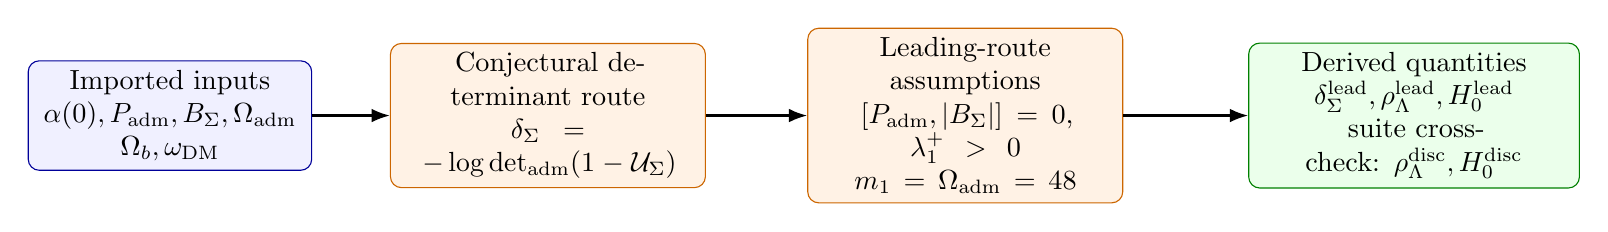
\begin{tikzpicture}[
    x=1cm,
    y=1cm,
    >=Latex,
    imported/.style={draw=blue!60!black, fill=blue!6, rounded corners, minimum width=3.6cm, minimum height=1.35cm, text width=3.3cm, align=center},
    conjectural/.style={draw=orange!80!black, fill=orange!10, rounded corners, minimum width=4.0cm, minimum height=1.35cm, text width=3.7cm, align=center},
    derived/.style={draw=green!50!black, fill=green!8, rounded corners, minimum width=4.2cm, minimum height=1.35cm, text width=3.9cm, align=center}
]
\node[imported] (a) at (0,0) {Imported inputs\\ $\alpha(0),\Padm,B_{\Seam},\Oadm$\\ $\Omega_b,\omegadm$};
\node[conjectural] (b) at (4.8,0) {Conjectural determinant route\\ $\delta_{\Seam}=-\log\det_{\mathrm{adm}}(1-\USeam)$};
\node[conjectural] (c) at (10.1,0) {Leading-route assumptions\\ $[\Padm,|B_{\Seam}|]=0$, $\lambda_1^+>0$\\ $m_1=\Oadm=48$};
\node[derived] (d) at (15.8,0) {Derived quantities\\ $\delta_{\Seam}^{\mathrm{lead}},\rhoLambda^{\mathrm{lead}},H_0^{\mathrm{lead}}$\\ suite cross-check: $\rhoLambda^{\mathrm{disc}},H_0^{\mathrm{disc}}$};
\draw[->, thick] (a) -- (b);
\draw[->, thick] (b) -- (c);
\draw[->, thick] (c) -- (d);
\end{tikzpicture}}
\caption{Status panel for the Letter. Imported benchmark/suite inputs feed the conjectural seam-determinant route; the leading Fredholm estimate additionally uses the admissible-branch reduction/no-zero-mode assumption and the imported identification $m_1=\Oadm=48$.}
\label{fig:mechanism-panel}
\end{figure*}

\section{Late-Time Hubble Closure}

At this stage the Letter needs more than the vacuum-sector inputs alone: the late-time Hubble closure also requires imported late-time matter quantities,
\begin{equation}
\Omega_b=0.04894,
\qquad
\omegadm=0.12275,
\qquad
h:=H_0/100.
\label{eq:matter-inputs}
\end{equation}
which are treated here as fixed imported values rather than as rederived outputs. In particular, $\Omega_b$ is the benchmark-side baryon fraction carried over from the companion manuscript's seed/Planck comparison layer, while $\omegadm$ is the TFPT suite dark-matter density parameter used in the late-time closure ledger.
With the standard conversion
\[
\kappa_H=2.133\times10^{-44}\,
\frac{\mathrm{GeV}}{\mathrm{km\,s^{-1}\,Mpc^{-1}}},
\qquad
H_0^{\mathrm{GeV}}=\kappa_H H_0,
\]
the flat late-time closure reads
\begin{equation}
\rhoLambda
=
3\Mplred^2(100\kappa_H)^2h^2
\left(1-\Omega_b-\frac{\omegadm}{h^2}\right).
\label{eq:friedmann}
\end{equation}
Equivalently,
\begin{equation}
A:=3\Mplred^2(100\kappa_H)^2,
\qquad
h^2
=
\frac{\omegadm+\rhoLambda/A}{1-\Omega_b}.
\label{eq:h2-closed}
\end{equation}
This closed formula is the cleanest way to discipline the Hubble discussion: once a late-time density is specified, the self-consistent $h^2$ value is fixed immediately.

\begin{figure*}[t]
\centering
\resizebox{0.94\textwidth}{!}{%
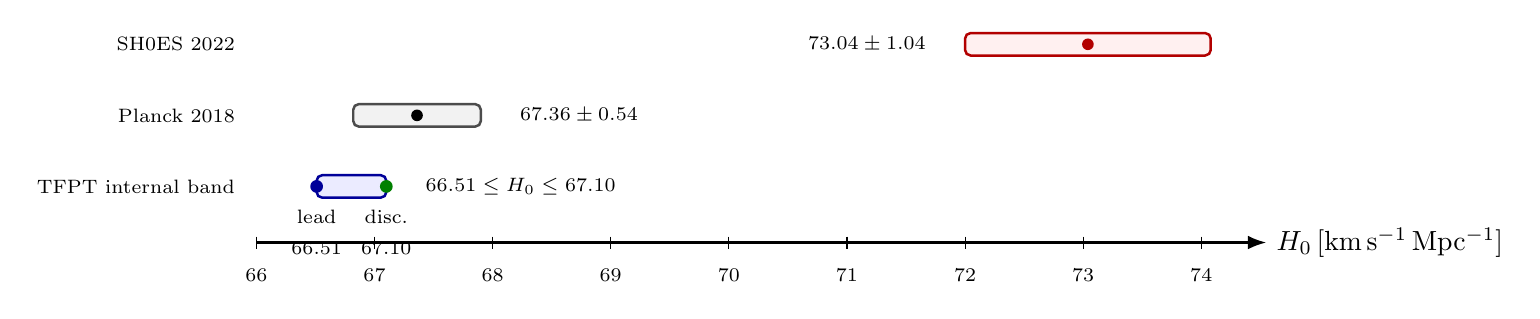
\begin{tikzpicture}[
    x=1.50cm,
    y=0.95cm,
    >=Latex,
    band/.style={rounded corners=2pt, line width=0.9pt}
]
\draw[->, thick] (0,0) -- (8.55,0) node[right] {$H_0\,[\mathrm{km\,s^{-1}\,Mpc^{-1}}]$};
\foreach \x/\lab in {0/66,1/67,2/68,3/69,4/70,5/71,6/72,7/73,8/74}{
  \draw (\x,0.08) -- (\x,-0.08);
  \node[below=4pt] at (\x,-0.08) {\scriptsize \lab};
}
\node[anchor=east] at (-0.10,0.75) {\scriptsize TFPT internal band};
\draw[band, draw=blue!60!black, fill=blue!8] (0.51,0.60) rectangle (1.10,0.90);
\fill[blue!60!black] (0.51,0.75) circle (2.3pt);
\fill[green!50!black] (1.10,0.75) circle (2.3pt);
\node[anchor=north, align=center] at (0.51,0.56) {\scriptsize lead\\[-1pt]\scriptsize 66.51};
\node[anchor=north, align=center] at (1.10,0.56) {\scriptsize disc.\\[-1pt]\scriptsize 67.10};
\node[anchor=west] at (1.35,0.75) {\scriptsize $66.51\le H_0\le67.10$};

\node[anchor=east] at (-0.10,1.70) {\scriptsize Planck 2018};
\draw[band, draw=black!70, fill=black!5] (0.82,1.55) rectangle (1.90,1.85);
\fill[black] (1.36,1.70) circle (2.1pt);
\node[anchor=west] at (2.15,1.70) {\scriptsize $67.36\pm0.54$};

\node[anchor=east] at (-0.10,2.65) {\scriptsize SH0ES 2022};
\draw[band, draw=red!70!black, fill=red!6] (6.00,2.50) rectangle (8.08,2.80);
\fill[red!70!black] (7.04,2.65) circle (2.1pt);
\node[anchor=east] at (5.75,2.65) {\scriptsize $73.04\pm1.04$};
\end{tikzpicture}}
\caption{Late-time closure panel. The TFPT lead and discrete routes define a narrow internal band close to the Planck interval and far below SH0ES. Under the same self-consistent closure map, a SH0ES-sized background would require $\rho_\Lambda^{\mathrm{SH0ES}}=3.11\times10^{-47}\,\mathrm{GeV}^4=1.259\,\rho_\Lambda^{\mathrm{disc}}$, i.e.\ a $25.9\%$ upward shift.}
\label{fig:h0-panel}
\end{figure*}

Applying Eq.~\eqref{eq:h2-closed} to the two TFPT density routes gives
\begin{equation}
\rhoLambda^{\mathrm{lead}}
\Rightarrow
H_0^{\mathrm{lead}}
=
66.51\,\mathrm{km\,s^{-1}\,Mpc^{-1}},
\label{eq:h0-lead}
\end{equation}
and
\begin{equation}
\rhoLambda^{\mathrm{disc}}
\Rightarrow
H_0^{\mathrm{disc}}
=
67.10\,\mathrm{km\,s^{-1}\,Mpc^{-1}}.
\label{eq:h0-disc}
\end{equation}
These correspond to
\[
(\Omega_{\mathrm{DM}},\Omega_{\Lambda})
=(0.27753,0.67353)
\quad\text{and}\quad
(0.27261,0.67845),
\]
respectively. The previous draft's quoted value $66.26\,\mathrm{km\,s^{-1}\,Mpc^{-1}}$ is not retained, because it came from a simple $\sqrt{\rho}$ rescaling at fixed $\Omega_{\Lambda}$ rather than from the self-consistent closure \eqref{eq:h2-closed}. The corrected self-consistent Fredholm-leading value is therefore Eq.~\eqref{eq:h0-lead}.
Combined with the positivity remark after Eq.~\eqref{eq:lead-densities}, the same closure map also implies that the exact Fredholm determinant route must satisfy $H_0>H_0^{\mathrm{lead}}=66.51\,\mathrm{km\,s^{-1}\,Mpc^{-1}}$.

Against the external benchmarks, the two TFPT routes therefore give
\[
z_{\mathrm{Planck}}^{\mathrm{lead}}=-1.58,
\qquad
z_{\mathrm{Planck}}^{\mathrm{disc}}=-0.48,
\]
and
\[
z_{\mathrm{SH0ES}}^{\mathrm{lead}}=-6.28,
\qquad
z_{\mathrm{SH0ES}}^{\mathrm{disc}}=-5.71.
\]
So the Fredholm-leading and discrete routes lie $1.58\sigma$ and $0.48\sigma$ below Planck, respectively, while remaining $6.28\sigma$ and $5.71\sigma$ below SH0ES. The sharpened conclusion is therefore not that TFPT predicts one magic number for $H_0$, but that the asymptotic background selected by its cosmological-constant sector is stably CMB-sized and clearly non-SH0ES-sized.

\begin{table}[b]
\small
\caption{Imported inputs, leading outputs, cross-check values, and benchmarks.}
\begin{ruledtabular}
\begin{tabular}{lll}
Object & Value & Status \\
$\alpha^{-1}(0)$ & $137.0359992$ & imported benchmark \\
$\Omega_b$ & $0.04894$ & imported benchmark-side \\
$\omegadm$ & $0.12275$ & imported suite input \\
$\delta_{\Seam}^{\mathrm{lead}}$ & $1.085\times10^{-123}$ & Fredholm lead \\
$\rhoLambdaRed^{\mathrm{lead}}$ & $3.81\times10^{-50}$ & Fredholm lead \\
$\rhoLambda^{\mathrm{lead}}$ & $2.41\times10^{-47}$ & Fredholm lead \\
$\rhoLambda^{\mathrm{disc}}$ & $2.4723\times10^{-47}$ & suite cross-check \\
$H_0^{\mathrm{lead}}$ & $66.51$ & derived from lead route \\
$H_0^{\mathrm{disc}}$ & $67.10$ & derived from cross-check \\
Planck 2018 & $67.36\pm0.54$ & benchmark \\
SH0ES 2022 & $73.04\pm1.04$ & benchmark \\
\end{tabular}
\end{ruledtabular}
\label{tab:claim-surface}
\end{table}

The resulting TFPT internal model band is therefore
\[
66.5 \lesssim H_0 \lesssim 67.1,
\]
with an internal spread
\[
\Delta\rho_\Lambda^{\mathrm{int}}\!/\,\rho_\Lambda
\approx 2.5\%,
\qquad
\Delta H_0^{\mathrm{int}}
\approx 0.60\,\mathrm{km\,s^{-1}\,Mpc^{-1}}.
\]
which remains much closer to Planck than to SH0ES. A SH0ES-sized asymptotic background would require, under the same self-consistent closure map,
\begin{equation}
\begin{aligned}
\rhoLambda^{\mathrm{SH0ES}}
&=
A\Bigl[(1-\Omega_b)\Bigl(\frac{73.04}{100}\Bigr)^2-\omegadm\Bigr]\\
&\approx
3.11\times10^{-47}\,\mathrm{GeV}^4,\\[2pt]
\frac{\rhoLambda^{\mathrm{SH0ES}}}{\rhoLambda^{\mathrm{disc}}}
&\approx
1.259,
\end{aligned}
\label{eq:sh0es-ratio}
\end{equation}
i.e. an approximately $25.9\%$ larger late-time vacuum density. That required shift is much larger than the $2.5\%$ spread between the Fredholm-leading density and the independent discrete suite route. Within this framework the Hubble tension is therefore not resolved by dialing the asymptotic vacuum scale upward. The central physical statement of the Letter is instead the shorter chain
\[
\alpha(0)
\longrightarrow
S_{\Seam}
\longrightarrow
\delta_{\Seam}^{\mathrm{lead}}
\longrightarrow
\rhoLambda
\longrightarrow
H_0 \ \text{near the CMB value}.
\]

\begin{thebibliography}{99}

\bibitem{tfpt31}
S.~Hamann and A.~Rizzo,
\emph{TFPT: Carrier Algebra, Closure Theorems, and Benchmark Bridge},
companion long-form manuscript (2026).

\bibitem{connes1997}
A.~H.~Chamseddine and A.~Connes,
\emph{The spectral action principle},
Commun.\ Math.\ Phys.\ \textbf{186} (1997), 731--750.

\bibitem{simon2005}
B.~Simon,
\emph{Trace Ideals and Their Applications},
2nd ed., Mathematical Surveys and Monographs \textbf{120}, American Mathematical Society (2005).

\bibitem{einstein1917}
A.~Einstein,
\emph{Kosmologische Betrachtungen zur allgemeinen Relativit\"atstheorie},
Sitzungsber.\ Preuss.\ Akad.\ Wiss.\ Berlin (1917), 142--152.

\bibitem{weinberg1989}
S.~Weinberg,
\emph{The cosmological constant problem},
Rev.\ Mod.\ Phys.\ \textbf{61} (1989), 1--23.

\bibitem{codata2022}
P.~J.~Mohr, D.~B.~Newell, and B.~N.~Taylor,
\emph{CODATA recommended values of the fundamental physical constants: 2022 update},
NIST / CODATA reference set, \url{https://physics.nist.gov/cuu/Constants/}, accessed March 2026.

\bibitem{planck2018}
Planck Collaboration,
\emph{Planck 2018 results. VI. Cosmological parameters},
Astron.\ Astrophys.\ \textbf{641} (2020), A6.

\bibitem{riess2022}
A.~G.~Riess \textit{et al.},
\emph{A Comprehensive Measurement of the Local Value of the Hubble Constant with 1 km s$^{-1}$ Mpc$^{-1}$ Uncertainty from the Hubble Space Telescope and the SH0ES Team},
Astrophys.\ J.\ Lett.\ \textbf{934} (2022), L7.

\end{thebibliography}

\end{document}
